%==============================================================================
%  LocalRCA -- IEEE conference format (IEEEtran)
%
%  Build:
%     pdflatex localrca_ieee
%     bibtex   localrca_ieee      % only if you switch to a .bib file
%     pdflatex localrca_ieee
%     pdflatex localrca_ieee
%
%  Self-contained: every figure is TikZ/pgfplots, so there are no external
%  image dependencies. Numbers in the figures are the measured values quoted
%  in the text; they are not illustrative.
%==============================================================================
\documentclass[conference,a4paper]{IEEEtran}
\IEEEoverridecommandlockouts

\usepackage{cite}
\usepackage{amsmath,amssymb,amsfonts}
\usepackage{algorithmic}
\usepackage{graphicx}
\usepackage{textcomp}
\usepackage{xcolor}
\usepackage{booktabs}
\usepackage{url}
\usepackage{tikz}
\usepackage{pgfplots}
\pgfplotsset{compat=1.17}
\usetikzlibrary{shapes.geometric, arrows.meta, positioning, calc, fit}

\def\BibTeX{{\rm B\kern-.05em{\sc i\kern-.025em b}\kern-.08em
    T\kern-.1667em\lower.7ex\hbox{E}\kern-.125emX}}

%--- diagram styles -----------------------------------------------------------
\tikzset{
  proc/.style   = {rectangle, rounded corners=2pt, draw, thick,
                   minimum width=22mm, minimum height=8mm, align=center,
                   font=\scriptsize},
  store/.style  = {cylinder, shape border rotate=90, aspect=0.25, draw, thick,
                   minimum width=16mm, minimum height=10mm, align=center,
                   font=\scriptsize},
  flowstep/.style = {rectangle, draw, thick, minimum width=30mm,
                   minimum height=7mm, align=center, font=\scriptsize},
  gate/.style   = {diamond, draw, thick, aspect=2.2, inner sep=1pt,
                   align=center, font=\scriptsize},
  term/.style   = {rectangle, rounded corners=8pt, draw, thick,
                   minimum width=24mm, minimum height=7mm, align=center,
                   font=\scriptsize},
  flow/.style   = {-{Stealth[length=2mm]}, thick},
  subsys/.style = {circle, draw, thick, minimum size=9mm, font=\scriptsize},
}

% Shrink-to-fit, never enlarge. Several diagrams are laid out in millimetres
% and come out wider than the 88.9mm IEEE column -- the architecture diagram
% spans ~97mm, the topology chain ~97mm -- so they bled into the neighbouring
% column. A plain \resizebox{\columnwidth} would also *stretch* the narrow
% ones, and the pipeline flowchart is already tall enough that scaling it up
% by half would push it off the page.
\newcommand{\fitcol}[1]{%
  \resizebox{\ifdim\width>\columnwidth\columnwidth\else\width\fi}{!}{#1}}

\def\IEEEkeywordsname{Keywords}
\makeatletter
% Break author blocks onto a second row (template: left to right, then down).
\newcommand{\linebreakand}{\end{@IEEEauthorhalign}\hfill\mbox{}\par
  \mbox{}\hfill\begin{@IEEEauthorhalign}}
\makeatother
\begin{document}

\title{LocalRCA: On-Device Root Cause Analysis for Windows Endpoints Without
Ground Truth}

\author{
\IEEEauthorblockN{Anonymous Authors}
\IEEEauthorblockA{Affiliation withheld for double-blind review}
}

\maketitle

\begin{abstract}
Diagnosing why a single Windows machine slowed down or failed is poorly served
by fleet observability tools, which assume a network, a backend and consent to
export telemetry. We present LocalRCA, a desktop system that records telemetry
without sending any of it off the machine, learns that machine's normal
behaviour with an LSTM autoencoder, and explains anomalies with Granger
causality constrained by false-discovery-rate control, an effect-size floor and
a subsystem topology prior. A personal machine has no labelled incidents, so we
evaluate with seven controlled fault injections and a replay over 596 incidents
found in real collected history. The system detects and correctly attributes
injected CPU, disk and memory faults, and in one case explained a fault it was
never told about. On real history it produces a supported causal chain for
106 of 596 incidents (17.8 percent, 95 percent confidence interval 14.9 to
21.1 percent), while 36 percent are too short to test. When it does answer, its top cause differs from the most
anomalous metric about half the time. The
hand-written subsystem prior rejects 22.7 percent of statistically accepted pairs,
including mechanisms that demonstrably exist. We argue that the most useful
property of such a tool is saying when it cannot explain an incident.
\end{abstract}

\begin{IEEEkeywords}
root cause analysis, anomaly detection, LSTM autoencoder, Granger causality,
endpoint telemetry, false discovery rate, explainability
\end{IEEEkeywords}

%==============================================================================
\section{Introduction}
%==============================================================================

Diagnosing why a personal computer became slow, stalled or crashed is
typically a manual exercise: an engineer lines up resource graphs against the
Windows Event Log and guesses. Fleet-oriented observability platforms automate
this, but they assume infrastructure a single machine does not have: a
collector network, a time-series backend, and the user's consent to export
telemetry that shows which applications they run.

Targeting a single endpoint imposes three constraints, and most of the design
follows from them.

\textbf{No egress.} Telemetry about application usage is sensitive, so the
system transmits nothing. The collector contains no network code, which means
privacy does not depend on a setting that someone could change.

\textbf{No ground truth.} A personal machine has no labelled incidents. The
model cannot be trained to recognise known faults and cannot be evaluated
against a labelled test set. This constraint shaped the evaluation more than
any other. The only workable response we found was to manufacture ground truth
by causing faults on purpose (Section~\ref{sec:eval}).

\textbf{Cold start is unavoidable.} ``Normal'' has to be learned from the
machine itself, so the tool can do nothing until it has seen enough normal
behaviour. In our configuration that takes about 10.5 hours of clean
collection.

Our contributions are:

\begin{enumerate}
  \item An end-to-end on-device RCA pipeline combining reconstruction-error
        anomaly detection with statistically constrained Granger causality
        (Section~\ref{sec:method}).
  \item A fault-injection harness that manufactures ground truth on a machine
        that has none, and a demonstration that the pipeline can identify a
        cause it was not told about (Section~\ref{sec:eval}).
  \item A population-scale measurement of how often the causal layer produces
        an answer at all, replicated on a second survey, and of how often
        that answer differs from simply naming the most anomalous metric
        (Section~\ref{sec:population}).
  \item An audit showing that the hand-written subsystem prior removes more
        statistically accepted pairs than any later stage of the pipeline, and
        that it forbids physically real mechanisms
        (Section~\ref{sec:topology}).
  \item A deployment design for a tool that holds sensitive telemetry
        (per-user encryption of the learned model, signed binaries, and an
        interface that separates the verdict from the evidence), including
        where it falls short (Section~\ref{sec:deploy}).
\end{enumerate}

%==============================================================================
\section{Related Work}
%==============================================================================

\textbf{Anomaly detection in multivariate time series.} Surveys of the
field~\cite{chandola2009survey, blazquez2021review} separate detectors by
whether labels exist and by whether the anomaly is a point, a subsequence or a
whole series. Reconstruction-based detectors built on LSTMs~\cite{hochreiter1997lstm}
are a standard approach when labelled anomalies are
unavailable~\cite{malhotra2016lstm, hundman2018detecting}. They train on
normal data only and threshold the reconstruction error, so they need no
labelled faults, which an endpoint does not have. Later detectors improve
accuracy with stochastic recurrent models
(OmniAnomaly~\cite{su2019omni}), adversarially trained autoencoders
(USAD~\cite{audibert2020usad}), signature matrices fed to convolutional LSTMs
(MSCRED~\cite{zhang2019mscred}), learned sensor graphs with attention
(GDN~\cite{deng2021gdn}) and transformers (TranAD~\cite{tuli2022tranad}).
MSCRED and GDN also point to the sensors responsible for an anomaly; none of
them says why those sensors moved. We keep the plain LSTM autoencoder because
its per-metric reconstruction error maps directly onto the metric to be
explained and it trains on a commodity CPU. Whether the heavier detectors
would pay for themselves on a single endpoint is not tested here.

\textbf{Log-based anomaly detection.} System logs are the other common
signal. Xu et al.~\cite{xu2009console} applied PCA to message-count vectors
mined from console logs, He et al.~\cite{he2016experience} benchmarked six
supervised and unsupervised log detectors, and DeepLog~\cite{du2017deeplog}
learns log-key sequences with an LSTM and flags keys it did not predict. On a
personal machine the Windows Event Log is sparse (our host logged
$6{,}600$ allow-listed records in 59 days), so LocalRCA uses it only as
context around a metric anomaly and not as a detector.

\textbf{Causal discovery from observational data.} Granger
causality~\cite{granger1969investigating} tests whether one series improves
prediction of another beyond the second's own history. It is correlational
under a temporal constraint rather than interventional, and is well known to
over-report on correlated series without correction. We apply
Benjamini--Hochberg false-discovery-rate control~\cite{benjamini1995controlling}
across the full set of ordered pairs, an effect-size floor, and a domain prior
over subsystems. Nonlinear extensions replace the linear autoregression with
neural networks whose sparse input weights identify Granger
causes~\cite{tank2022neural}, and PCMCI~\cite{runge2019pcmci} conditions on
each series' own past and a selected parent set to suppress false links caused
by autocorrelation. Both need longer series than an incident window usually
provides: Section~\ref{sec:population} shows that $36\%$ of real incidents are
too short even for the linear test.

\textbf{Root cause analysis in distributed systems.} Microservice RCA work
typically exploits service call graphs or distributed traces to constrain
candidate causes~\cite{kim2013root, chen2014causeinfer}, and Soldani and
Brogi~\cite{soldani2022survey} review how faults are found and traced in
cloud microservice deployments. Most methods first work out which component
depends on which and then traverse that structure.
CloudRanger~\cite{wang2018cloudranger} infers causal structure through
PC-based discovery and ranks candidates by a second-order random walk; AutoMAP~\cite{ma2020automap} builds behaviour graphs over several
metrics; MicroRCA~\cite{wu2020microrca} runs personalised PageRank over an
attributed service--host graph; and MicroCause~\cite{meng2020microcause} pairs
a PCMCI-derived causal graph with a temporal cause-oriented random walk.
CIRCA~\cite{li2022circa} derives a structural graph from the system
architecture and treats root-cause identification as recognising which
variable was intervened on, while BARO~\cite{pham2024baro} needs no graph and
ranks each metric by how sharply its distribution shifts, estimated with a
Bayesian change-point model. A
single endpoint has no service topology, so we write an explicit subsystem map
by hand, and Section~\ref{sec:topology} shows how much the quality of that map
then matters.

\textbf{Benchmarked causal RCA at fleet scale.} Recent work evaluates causal
discovery for root cause analysis at a scale this system does not attempt.
Ikram et al.~\cite{ikram2022root} discover root causes across thousands of
microservice nodes and report top-$k$ recall against ground truth gathered
from a real production incident corpus. Pham et al.~\cite{pham2024root}
benchmark six causal-RCA methods (including CausalRCA and BARO) across
microservice architectures and find that none dominates uniformly and that
results depend heavily on the call graph. Both assume a call graph or trace
corpus that a single endpoint does not have. Our work differs in running on
one machine, with no ground truth, and in reporting when it cannot explain an
incident instead of ranking whatever the evidence.

%==============================================================================
\section{System Architecture}
%==============================================================================

The system is two processes that share a SQLite database
(Fig.~\ref{fig:arch}). They are separate because collection has to keep
running after the user closes the interface.

\begin{figure}[t]
\centering
\fitcol{%
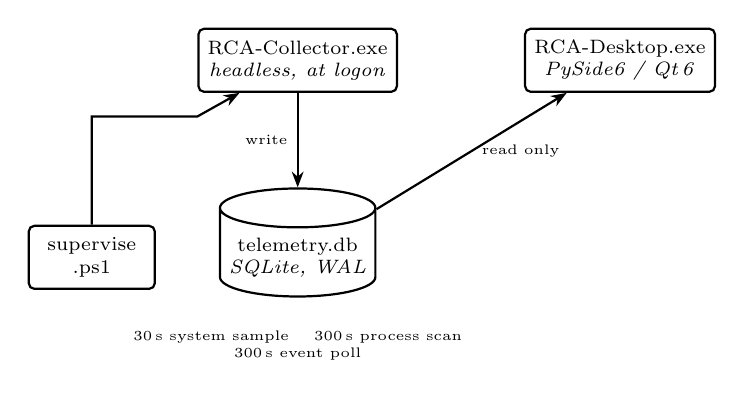
\begin{tikzpicture}[node distance=6mm]
  \node[proc] (coll) {RCA-Collector.exe\\\textit{headless, at logon}};
  \node[store, below=12mm of coll] (db) {telemetry.db\\\textit{SQLite, WAL}};
  \node[proc, right=16mm of coll] (gui) {RCA-Desktop.exe\\\textit{PySide6 / Qt\,6}};
  \node[proc, left=8mm of db, minimum width=16mm] (sup) {supervise\\.ps1};

  \draw[flow] (coll) -- node[left, font=\tiny] {write} (db);
  \draw[flow] (db) -- node[right, font=\tiny] {read only} (gui);
  \draw[flow] (sup) |- ([yshift=-3mm]coll.south west) -- (coll);

  \node[font=\tiny, align=center, below=3mm of db] {%
    30\,s system sample \quad 300\,s process scan\\ 300\,s event poll};
\end{tikzpicture}}
\caption{Process architecture. The collector writes; the desktop application
only reads. A PowerShell supervisor restarts the collector without needing
administrator rights.}
\label{fig:arch}
\end{figure}

The collector records 29 channels every 30 seconds, the top processes by CPU
and resident memory every 300 seconds (tightening to 30 seconds under load),
and an allow-listed subset of Windows Event Log records. Retention is
tiered by sensitivity: numeric readings for 365 days, per-process detail for
30 days, and the foreground application name, the most personal field
collected, for 30 days.

The evaluation host is a laptop with an Intel Core i7-14700HX (28 logical
processors) and 16\,GB of RAM, running Windows 11 Home. At the time of the
first survey it had accumulated $124{,}674$ system
samples, $1{,}835{,}250$ process samples and $6{,}600$ Event Log records over
59 days, occupying 227\,MB. Coverage of that span is $73.1\%$: 157 breaks in
collection account for 383 hours not recorded. The population survey
(Section~\ref{sec:population}) draws on the most recent 30 days of this
history.

Collection is cheap but not free. Measured over 5- and 15-minute windows,
the collector used 14--21\% of one logical processor ($0.5$--$0.7\%$ of the
host's capacity) with a 16\,MB working set. Across $133{,}753$ samples the
spacing had a median of $30.0$\,s and a 99th percentile of $30.005$\,s, so
the cost does not delay sampling.

%==============================================================================
\section{Method}
\label{sec:method}
%==============================================================================

\subsection{Scaling and windowing}

A min--max scaler is fitted on the clean baseline only,
$x'_j = (x_j - \min_j)/(\max_j - \min_j)$, and incident windows are transformed
with the baseline's parameters and clipped to $[0,1]$. Fitting on the incident
would normalise away the deviation being sought.

Training windows are built \emph{within contiguous segments only}, never
spanning a collection gap. A segment is a maximal run of samples whose spacing
is within tolerance of the sampling cadence.

\subsection{Anomaly detection}

An LSTM autoencoder compresses a window of $T=12$ samples (six minutes) over
$n=17$ features to a 32-dimensional latent vector and reconstructs it. The 17
are the numeric resource metrics the host reports; the other recorded
channels are raw counters, GPU and idle readings, the foreground application,
and two battery fields that are empty on this host, and are not modelled. Only the encoder's final
hidden state reaches the bottleneck, so the entire window is represented by 32
numbers before reconstruction; that compression is the detection mechanism.
Encoder and decoder are two-layer LSTMs with 64 hidden units and dropout
$0.2$ ($126{,}385$ parameters). Training minimises
\begin{equation}
\mathcal{L} = \frac{1}{B\,T\,n}\sum_{b,t,j}\bigl(x_{btj}-\hat{x}_{btj}\bigr)^2 .
\end{equation}

Error is reduced over time but \emph{not} over features, which is what makes
the output attributable to a metric rather than to a window:
\begin{equation}
s_j = \frac{1}{T}\sum_{t=1}^{T}\bigl(x_{tj}-\hat{x}_{tj}\bigr)^2 .
\end{equation}

We train with Adam (learning rate $10^{-3}$, batch 32) for five epochs on
windows taken at stride 5 within clean segments, hold out the last 20\% of
windows in time order for validation, and keep the epoch with the lowest
validation loss. Training starts once 250 windows exist, which is the
10.5 hours quoted above. Per-metric thresholds are the 99th percentile of
validation error,
$\tau_j = P_{99}\{s_j(w)\}$, and a metric is anomalous when $s_j > \tau_j$.
Per-metric thresholds are necessary because reconstructability varies widely:
a near-constant channel reconstructs almost perfectly, while a bursty one does
not, and a single global threshold would flag the latter permanently. By
construction about 1\% of normal windows exceed each threshold, so an
incident needs at least three consecutive flagged samples.

\subsection{Constrained causal inference}

For each ordered pair of anomalous metrics, both series are differenced until
an Augmented Dickey--Fuller test~\cite{dickey1979distribution} rejects a unit
root (at most twice), then
tested for Granger causality at lags $1\ldots L$. The lag minimising the
$p$-value is selected. A pair is skipped unless
\begin{equation}
N \;\ge\; 3L + 2 ,
\label{eq:floor}
\end{equation}
which at the default $L=5$ requires 17 aligned samples. Most of this
system's negative results come from Equation~\eqref{eq:floor}.

Surviving $p$-values are corrected with Benjamini--Hochberg: sorting ascending,
the largest rank $k$ satisfying $p_{(k)} \le \alpha k / m$ is found and ranks
$1\ldots k$ accepted, with $\alpha = 0.05$. A $p$-value alone is not enough,
because with a long history even a negligible improvement becomes significant,
so we also require an effect-size proxy:
\begin{equation}
\mathrm{effect} = \frac{F}{F+N} \;\ge\; 0.10 .
\end{equation}
This quantity is monotone in $F$, lies in $(0,1)$, and shrinks as $N$ grows.
That is the correction we want, since a large $N$ is what made the $p$-value
small.

Accepted pairs form a directed graph; cycles are removed preferring edges that
contradict temporal precedence, and remaining edges are filtered against a
subsystem topology prior (Section~\ref{sec:topology}). Candidates are then
ranked by a weighted composite plus PageRank~\cite{page1999pagerank} on the
reversed graph:
\begin{equation}
\mathrm{score}(v) = \min\!\Bigl(1,\; 0.70\!\sum_k w_k s_k(v) \;+\; 0.30\,\mathrm{PR}(v)\Bigr),
\end{equation}
with weights $0.40$ causal outflow, $0.30$ temporal priority, $0.20$ low
inflow, $0.05$ severity and $0.05$ event correlation.

\textbf{A structural caveat.} With zero surviving edges, every node has
outflow $0$ and inflow $1$, so $60\%$ of the weight becomes constant and the
ranking collapses onto severity and timing while still emitting a score. The
system therefore reports the distinction explicitly rather than presenting the
ranking as causal.

\begin{figure}[t]
\centering
\fitcol{%
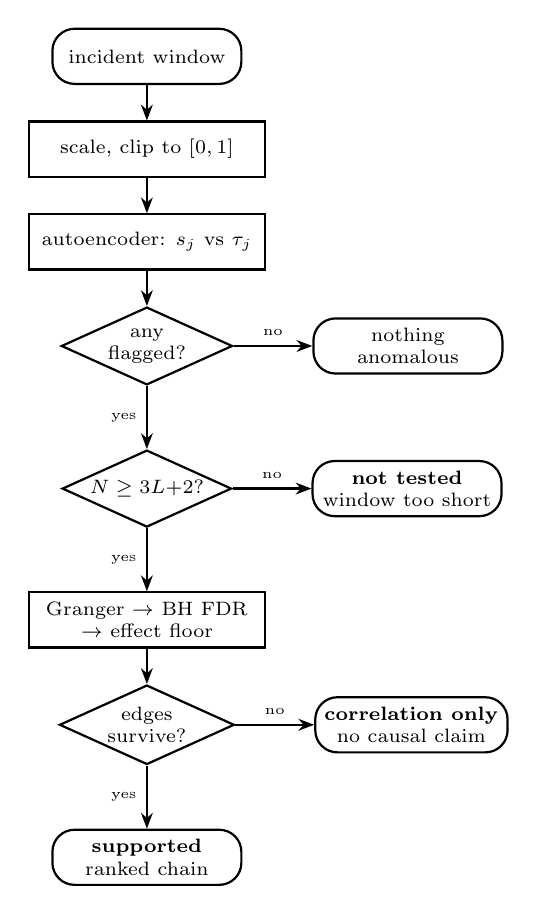
\begin{tikzpicture}[node distance=4.5mm]
  \node[term] (start) {incident window};
  \node[flowstep, below=of start] (scale) {scale, clip to $[0,1]$};
  \node[flowstep, below=of scale] (score) {autoencoder: $s_j$ vs $\tau_j$};
  \node[gate, below=of score, minimum width=20mm] (any) {any\\flagged?};
  \node[term, right=10mm of any] (none) {nothing\\anomalous};
  \node[gate, below=8mm of any, minimum width=20mm] (floor) {$N \ge 3L{+}2$?};
  \node[term, right=10mm of floor] (untested) {\textbf{not tested}\\window too short};
  \node[flowstep, below=8mm of floor] (granger) {Granger $\rightarrow$ BH FDR\\$\rightarrow$ effect floor};
  \node[gate, below=of granger, minimum width=20mm] (edges) {edges\\survive?};
  \node[term, right=10mm of edges] (corr) {\textbf{correlation only}\\no causal claim};
  \node[term, below=8mm of edges] (ok) {\textbf{supported}\\ranked chain};

  \draw[flow] (start) -- (scale);
  \draw[flow] (scale) -- (score);
  \draw[flow] (score) -- (any);
  \draw[flow] (any) -- node[above, font=\tiny] {no} (none);
  \draw[flow] (any) -- node[left, font=\tiny] {yes} (floor);
  \draw[flow] (floor) -- node[above, font=\tiny] {no} (untested);
  \draw[flow] (floor) -- node[left, font=\tiny] {yes} (granger);
  \draw[flow] (granger) -- (edges);
  \draw[flow] (edges) -- node[above, font=\tiny] {no} (corr);
  \draw[flow] (edges) -- node[left, font=\tiny] {yes} (ok);
\end{tikzpicture}}
\caption{Inference pipeline. Four end states are reported separately, so
``not tested'' is never shown as ``nothing survived''.}
\label{fig:pipeline}
\end{figure}

%==============================================================================
\section{Evaluation by Fault Injection}
\label{sec:eval}
%==============================================================================

Because a personal machine provides no labelled incidents, we manufacture
ground truth: a harness causes a specific, known disturbance, waits for
samples to land at the real cadence, runs the production pipeline over the
injection window, and scores the result.

\begin{table}[t]
\caption{Controlled fault injections, 30-minute windows unless noted.
Flagged counts are out of the 17 modelled metrics.}
\label{tab:injection}
\centering
\footnotesize
\fitcol{%
\begin{tabular}{@{}llccl@{}}
\toprule
\textbf{Fault} & \textbf{Samples} & \textbf{Flagged} & \textbf{Edges} & \textbf{Outcome} \\
\midrule
CPU, 7\,min      & 14 & 6/17 & --- & not tested (below floor) \\
CPU              & 60 & 6/17 & \textbf{6} & \textbf{explained correctly} \\
Disk             & 60 & 4/17 & 0 & detected, unexplained \\
Memory           & 60 & 2/17 & 0 & wrong process named \\
Memory (refixed) & 60 & 3/17 & 0 & detected, attributed \\
Memory (clean)   & 60 & 0/17 & --- & not measurable on host \\
Idle             & 60 & 1/17 & --- & 5.9\% false positives \\
\bottomrule
\end{tabular}}
\end{table}

\subsection{A correct explanation of an unknown cause}

Half the CPU cores were burned for 30 minutes with no information given to the
pipeline. The ranking named \texttt{cpu\_pct} first at $1.000$, and the
surviving edges point \emph{away} from CPU. That is what a real root cause
should look like, since nothing upstream drives it:
\[
\texttt{cpu\_pct\_max\_core} 
\rightarrow \texttt{disk\_busy\_pct}
\]
\[
(\text{lag } 2,\ 0.756).
\]

\subsection{Short windows starve the causal layer}

The same fault at 7 and at 30 minutes differed only in duration. At 14 samples,
against the floor of 17 from~\eqref{eq:floor}, \emph{no pair was compared at
all}, and the system reported exactly that. At 60 samples, ten pairs survived
correction and six survived the topology filter. The causal layer worked;
it was short of samples, so the fix is a wider window rather than a redesign.
Section~\ref{sec:population} confirms this at scale.

\subsection{A defect that injection exposed}

The memory injection detected the anomaly and then attributed it to four
unrelated processes. Attribution ranked candidates by mean CPU, while resident
memory was selected but never sorted on, so a process that allocates memory
and then sleeps could never be named. A memory-bound cause was unreportable
\emph{by construction} in every incident the system had ever analysed. The CPU
and disk faults are both CPU-heavy, so they happened to be attributed
correctly, and that hid the defect.

\subsection{A measurement this host cannot provide}

A later memory injection on a deliberately cleared machine flagged nothing.
The detector was correct: the host's median memory utilisation across 30{,}199
samples is $95.2\%$, and the injection window sat at $87.4\%$, the 9th
percentile of the host's own history. For safety the injection is limited to
half of free memory, and on a host that is usually full that cannot push usage
above the level the machine already reaches on its own. The fault is undetectable \emph{by construction} here,
and the harness now reports this as inconclusive rather than as a detector
failure.

%==============================================================================
\section{Population-Scale Evaluation}
\label{sec:population}
%==============================================================================

Fault injection establishes correctness on a handful of cases but yields single
observations. To measure \emph{frequency}, the pipeline was replayed over every
incident found in real collected history, read-only and with no injection.

\begin{figure}[t]
\centering
\fitcol{%
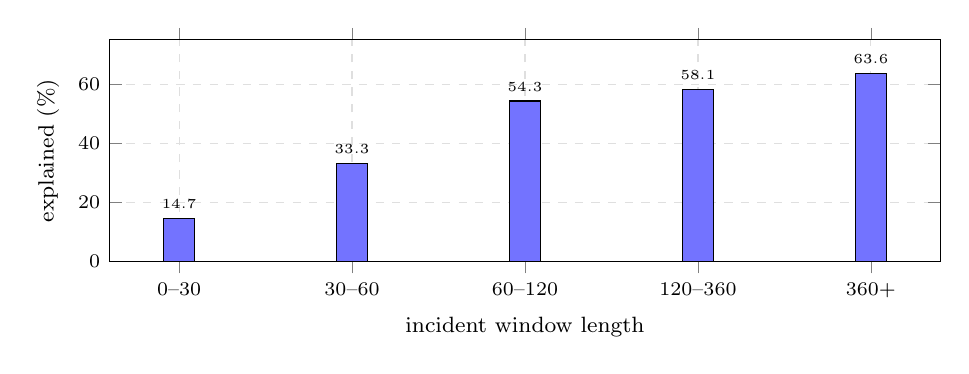
\begin{tikzpicture}
\begin{axis}[
  width=\columnwidth, height=4.4cm,
  ybar, bar width=11pt,
  ymin=0, ymax=75,
  ylabel={\footnotesize explained (\%)},
  xlabel={\footnotesize incident window length},
  symbolic x coords={0--30,30--60,60--120,120--360,360+},
  xtick=data,
  tick label style={font=\scriptsize},
  label style={font=\scriptsize},
  nodes near coords, every node near coord/.append style={font=\tiny},
  grid=major, grid style={dashed,gray!25},
]
\addplot[fill=blue!55] coordinates
  {(0--30,14.7) (30--60,33.3) (60--120,54.3) (120--360,58.1) (360+,63.6)};
\end{axis}
\end{tikzpicture}}
\caption{Causal yield against window length, over 381 analysable incidents
($L=5$, 30-day survey). The rate rises steadily with window length.}
\label{fig:yield}
\end{figure}

Of $596$ incidents discovered, $215$ ($36\%$) fall below the sample floor of
\eqref{eq:floor} and cannot be tested at any setting. Of the $381$ that can be,
$106$ produce a supported causal chain. The end-to-end figure a user experiences
is therefore $106/596 = 17.8\%$ (95\% Wilson interval $14.9$--$21.1\%$):
roughly one incident in six receives a causal explanation.

We report the whole funnel. Counting only \emph{analysable} incidents would
give $27.8\%$ ($23.6$--$32.5\%$), which looks better but describes fewer
situations.

\textbf{The floor is a parameter artefact.} Short incidents are widened before
analysis to exactly the model's window size, 12 samples (5.5 minutes), while
\eqref{eq:floor} at $L=5$ requires 17. The two constants were chosen independently in the same
pipeline.
Re-running the survey at $L\in\{3,4,5\}$ over an identical population (598
incidents discovered over 30 days of real collected history) confirms the
cliff disappears at $L\le3$: 0 incidents fall below the floor, versus 215 at
$L=5$. Explanations rise only modestly, from $106$ to $110$, while the tested
population nearly triples (381 to 598), and median surviving edges holds at
$2$ throughout. What improves is the reporting: more incidents read
``tested, nothing found'' instead of ``not tested'', but few gain an
explanation.

\textbf{Replication.} Four days later we re-ran the survey at $L=5$ on the
then most recent 30 days. The two windows share about 26 days, so this checks
stability rather than giving an independent sample. It found $520$
incidents, of which $177$ ($34.0\%$) fell below the floor and $94$ were
explained ($18.1\%$, $15.0$--$21.6\%$), in line with the first run.

\textbf{Does causality change the answer?} A ranking that always named the
most anomalous metric would need no causal layer. For each of the $94$
explained incidents we compared the top-ranked cause with the metric that had
the largest anomaly score. They agree in $46$ ($48.9\%$, $39.1$--$58.9\%$)
and fall in the same subsystem in $62$ ($66.0\%$). Where they differ, the
causal ranking most often puts a disk metric ahead of a pressure symptom, for
example \texttt{disk\_free\_pct} ahead of \texttt{swap\_used\_delta}.
This shows the causal ranking is not severity under another name. It does not
show the changed answer is the right one, which needs incidents with a known
cause.

%==============================================================================
\section{Auditing the Subsystem Prior}
\label{sec:topology}
%==============================================================================

Since no service call graph exists on an endpoint, the system encodes domain
knowledge as an explicit map of permissible subsystem influence. Auditing it
across all analysable incidents shows it is the largest single filter in the
pipeline after the statistical gates: of $538$ accepted pairs, $337$
($62.6\%$) survive, $122$ ($22.7\%$) are rejected by the map and $79$
($14.7\%$) by cycle-breaking.

\begin{figure}[t]
\centering
\fitcol{%
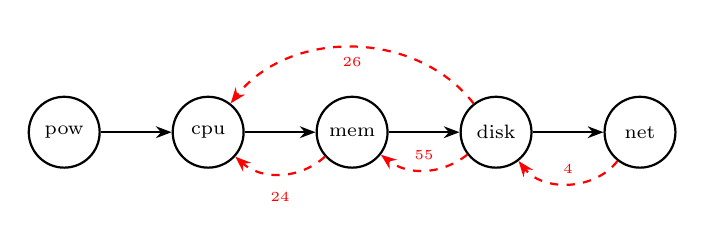
\begin{tikzpicture}[node distance=9mm]
  \node[subsys] (pow) {pow};
  \node[subsys, right=of pow] (cpu) {cpu};
  \node[subsys, right=of cpu] (mem) {mem};
  \node[subsys, right=of mem] (dsk) {disk};
  \node[subsys, right=of dsk] (net) {net};

  \draw[flow] (pow) -- (cpu);
  \draw[flow] (cpu) -- (mem);
  \draw[flow] (mem) -- (dsk);
  \draw[flow] (dsk) -- (net);

  \draw[flow, red, dashed] (dsk) to[bend left=38] node[above, font=\tiny] {55} (mem);
  \draw[flow, red, dashed] (mem) to[bend left=42] node[below=1mm, font=\tiny] {24} (cpu);
  \draw[flow, red, dashed] (net) to[bend left=52] node[above, font=\tiny] {4} (dsk);
  \draw[flow, red, dashed] (dsk) to[bend right=52] node[below, font=\tiny] {26} (cpu);
\end{tikzpicture}}
\caption{The subsystem prior is a strict total order (solid), so
\texttt{network} is a sink and nothing can be reported as caused by network
activity. Dashed edges are directions the statistics accepted and the map
rejected, labelled with occurrence counts (30-day, 596-incident survey).
Two of them describe real
mechanisms: the file cache consuming memory under write pressure, and
interrupt handling costing CPU during disk activity; a download writing to
disk (\texttt{network}$\rightarrow$\texttt{disk}) remains a smaller but
real third case.}
\label{fig:topology}
\end{figure}

Every rejected transition has \emph{zero} survivors, because the map forbids
whole classes rather than individual edges (Fig.~\ref{fig:topology}). Judged
individually, \texttt{disk}\,$\rightarrow$\,\texttt{memory} is almost certainly
real (the Windows standby file cache grows under write pressure) and is the
strongest single rejected relationship measured in this run, at $0.654$
(\texttt{disk\_write\_bps}$\rightarrow$\texttt{swap\_used\_delta}, lag 2).
\texttt{disk}\,$\rightarrow$\,\texttt{cpu}
reflects interrupt and DPC handling, and \texttt{network}\,$\rightarrow$\,
\texttt{disk} is the download-writes-to-disk case argued in the prior
revision of this analysis, present but smaller in this run (4 occurrences).
Conversely, the smallest rejected classes
(\texttt{network}$\rightarrow$\texttt{process},
\texttt{disk}$\rightarrow$\texttt{process}, at 1--2 occurrences each) are
plausibly spurious rather than real mechanisms being wrongly forbidden.

The prior only runs one way: it models pressure flowing downhill and cannot
express the feedback that makes I/O expensive. Adding reverse edges would make
it cyclic, and cycle-breaking already removes $14.7\%$ of pairs, so we leave
this as an open question rather than patch it.

%==============================================================================
\section{Deployment Engineering}
\label{sec:deploy}
%==============================================================================

A research prototype can leave its data in plaintext and show its results as
raw tables. A tool that someone else installs, and that records when and how
they use their machine, should not. This section describes what the released
application (v1.5.2) does about both problems and where it falls short.

\subsection{Protecting the model at rest}

The trained model holds per-metric bounds and thresholds, a compact profile
of how the machine is used. It is wrapped with the Windows Data Protection
API (DPAPI), which binds it to the user's logon, and written atomically.
The database and logs rely on the Encrypting File System (EFS), which does
not exist on Windows Home. The evaluation host runs Home, so its 227\,MB
database is in plaintext, protected only by file permissions, and its model,
trained before encryption was added, stays plaintext until retrained. Review
also found that an interrupted training run left a plaintext checkpoint on
disk; it is now removed in a \texttt{finally} block.

\subsection{Signed binaries}

Both executables are Authenticode-signed and timestamped, and each release
publishes a SHA-256 checksum. The certificate is self-signed, so it proves a
binary is unchanged but not who built it, and Windows SmartScreen still warns
on first run.

\subsection{Separating the verdict from the evidence}

The first screen used to show every captured channel with its raw value, and
stated training readiness four different ways. Hiding this would contradict
the project's premise, since a user cannot consent to collection they cannot
inspect.

The released interface shows the same computation two ways, chosen by one
switch that is off by default. The simple view opens each tab with a single
coloured sentence (for example, \emph{Healthy} only at $\ge 90\%$ coverage
with at most three breaks) and opens inference on the plain-language report.
The advanced view adds the raw counts, channel table, hyperparameters, lag
and score columns. Both views read the same figures; only presentation
changes.

This design has been checked by one expert review, not with users.

%==============================================================================
\section{Discussion and Threats to Validity}
%==============================================================================

\textbf{All measurements come from one machine.} Nothing here shows that the
results generalise. One measurement, memory-fault detection, cannot be made on
this host at all, so testing on a second machine is required, not optional.

\textbf{Correctness is not established at population scale.} The survey's 596
incidents have no known cause, so the $17.8\%$ explanation rate says how often
the causal layer gives an answer, not whether the answer is right. It is an
upper bound on usefulness rather than a measure of accuracy. For the same
reason we report no precision, recall or F1 for the detector: seven injected
windows show that detection works, not how often.

\textbf{No fault has been tested whose cause is not also the loudest metric.}
Both explaining runs put the injected fault atop a severity ranking, so a
correct causal answer and a correct severity answer remain indistinguishable.
On real incidents the two rankings differ about half the time
(Section~\ref{sec:population}), but none of those incidents has a known
cause.

\textbf{Granger causality is not causation.} It is correlation under a temporal
constraint; the FDR correction, effect floor and prior limit over-reporting.

\textbf{A methodological observation.} Adversarial review found nine defects
that a passing 130-test suite missed, because each test checked something next
to what mattered. The suite now has 195 tests.

%==============================================================================
\section{Conclusion}
%==============================================================================

We presented an on-device root cause analysis system for Windows endpoints
operating without ground truth, network access or fleet context. Under
controlled injection it detects and attributes CPU, disk and memory faults, and
has produced a correct causal explanation of a fault it was never told about.
Across real history it explains roughly one incident in six, declines to
explain the rest, and distinguishes ``not tested'' from ``tested and nothing
survived''.

We argue this last property matters more than the explanation rate: saying
``no causal chain was supported'' is more useful than a confident ranking that
changes with the analysis window.

Future work: a second machine, a fault whose cause is not the loudest metric,
a prior that admits feedback directions, database encryption without EFS, and
a user study of the default view.

The source code, fault-injection harness and survey scripts are public at
a public repository (link withheld for double-blind review). The collected
telemetry is not released, because it records one person's application use.

%==============================================================================
\begin{thebibliography}{00}

\bibitem{chandola2009survey}
V.~Chandola, A.~Banerjee, and V.~Kumar, ``Anomaly detection: A survey,''
\emph{ACM Comput. Surv.}, vol.~41, no.~3, pp. 1--58, 2009.

\bibitem{blazquez2021review}
A.~Bl\'{a}zquez-Garc\'{i}a, A.~Conde, U.~Mori, and J.~A. Lozano, ``A review on
outlier/anomaly detection in time series data,'' \emph{ACM Comput. Surv.},
vol.~54, no.~3, pp. 1--33, 2021.

\bibitem{hochreiter1997lstm}
S.~Hochreiter and J.~Schmidhuber, ``Long short-term memory,'' \emph{Neural
Comput.}, vol.~9, no.~8, pp. 1735--1780, 1997.

\bibitem{malhotra2016lstm}
P.~Malhotra, A.~Ramakrishnan, G.~Anand, L.~Vig, P.~Agarwal, and G.~Shroff,
``LSTM-based encoder-decoder for multi-sensor anomaly detection,'' in
\emph{Proc. ICML Anomaly Detection Workshop}, 2016.

\bibitem{hundman2018detecting}
K.~Hundman, V.~Constantinou, C.~Laporte, I.~Colwell, and T.~Soderstrom,
``Detecting spacecraft anomalies using LSTMs and nonparametric dynamic
thresholding,'' in \emph{Proc. ACM SIGKDD}, 2018, pp. 387--395.

\bibitem{su2019omni}
Y.~Su, Y.~Zhao, C.~Niu, R.~Liu, W.~Sun, and D.~Pei, ``Robust anomaly detection
for multivariate time series through stochastic recurrent neural network,'' in
\emph{Proc. 25th ACM SIGKDD Int. Conf. Knowl. Discovery Data Mining}, 2019,
pp. 2828--2837.

\bibitem{audibert2020usad}
J.~Audibert, P.~Michiardi, F.~Guyard, S.~Marti, and M.~A. Zuluaga, ``USAD:
UnSupervised anomaly detection on multivariate time series,'' in \emph{Proc.
26th ACM SIGKDD Int. Conf. Knowl. Discovery Data Mining}, 2020,
pp. 3395--3404.

\bibitem{zhang2019mscred}
C.~Zhang, D.~Song, Y.~Chen, X.~Feng, C.~Lumezanu, W.~Cheng, J.~Ni, B.~Zong,
H.~Chen, and N.~V. Chawla, ``A deep neural network for unsupervised anomaly
detection and diagnosis in multivariate time series data,'' in \emph{Proc.
AAAI Conf. Artif. Intell.}, vol.~33, no.~1, 2019, pp. 1409--1416.

\bibitem{deng2021gdn}
A.~Deng and B.~Hooi, ``Graph neural network-based anomaly detection in
multivariate time series,'' in \emph{Proc. AAAI Conf. Artif. Intell.},
vol.~35, no.~5, 2021, pp. 4027--4035.

\bibitem{tuli2022tranad}
S.~Tuli, G.~Casale, and N.~R. Jennings, ``TranAD: Deep transformer networks
for anomaly detection in multivariate time series data,'' \emph{Proc. VLDB
Endow.}, vol.~15, no.~6, pp. 1201--1214, 2022.

\bibitem{xu2009console}
W.~Xu, L.~Huang, A.~Fox, D.~Patterson, and M.~I. Jordan, ``Detecting
large-scale system problems by mining console logs,'' in \emph{Proc. ACM
SIGOPS 22nd Symp. Operating Syst. Principles (SOSP)}, 2009, pp. 117--132.

\bibitem{he2016experience}
S.~He, J.~Zhu, P.~He, and M.~R. Lyu, ``Experience report: System log analysis
for anomaly detection,'' in \emph{Proc. IEEE 27th Int. Symp. Softw. Rel. Eng.
(ISSRE)}, 2016, pp. 207--218.

\bibitem{du2017deeplog}
M.~Du, F.~Li, G.~Zheng, and V.~Srikumar, ``DeepLog: Anomaly detection and
diagnosis from system logs through deep learning,'' in \emph{Proc. ACM SIGSAC
Conf. Comput. Commun. Secur. (CCS)}, 2017, pp. 1285--1298.

\bibitem{granger1969investigating}
C.~W.~J. Granger, ``Investigating causal relations by econometric models and
cross-spectral methods,'' \emph{Econometrica}, vol.~37, no.~3, pp. 424--438,
1969.

\bibitem{benjamini1995controlling}
Y.~Benjamini and Y.~Hochberg, ``Controlling the false discovery rate: a
practical and powerful approach to multiple testing,'' \emph{J. Roy. Statist.
Soc. B}, vol.~57, no.~1, pp. 289--300, 1995.

\bibitem{tank2022neural}
A.~Tank, I.~Covert, N.~Foti, A.~Shojaie, and E.~B. Fox, ``Neural Granger
causality,'' \emph{IEEE Trans. Pattern Anal. Mach. Intell.}, vol.~44,
no.~8, pp. 4267--4279, 2022.

\bibitem{runge2019pcmci}
J.~Runge, P.~Nowack, M.~Kretschmer, S.~Flaxman, and D.~Sejdinovic, ``Detecting
and quantifying causal associations in large nonlinear time series datasets,''
\emph{Sci. Adv.}, vol.~5, no.~11, Art. no. eaau4996, 2019.

\bibitem{kim2013root}
M.~Kim, R.~Sumbaly, and S.~Shah, ``Root cause detection in a service-oriented
architecture,'' in \emph{Proc. ACM SIGMETRICS}, 2013, pp. 93--104.

\bibitem{chen2014causeinfer}
P.~Chen, Y.~Qi, P.~Zheng, and D.~Hou, ``CauseInfer: automatic and distributed
performance diagnosis with hierarchical causality graph in large distributed
systems,'' in \emph{Proc. IEEE INFOCOM}, 2014, pp. 1887--1895.

\bibitem{soldani2022survey}
J.~Soldani and A.~Brogi, ``Anomaly detection and failure root cause analysis
in (micro) service-based cloud applications: A survey,'' \emph{ACM Comput.
Surv.}, vol.~55, no.~3, pp. 1--39, 2022.

\bibitem{wang2018cloudranger}
P.~Wang, J.~Xu, M.~Ma, W.~Lin, D.~Pan, Y.~Wang, and P.~Chen, ``CloudRanger:
Root cause identification for cloud native systems,'' in \emph{Proc. 18th
IEEE/ACM Int. Symp. Cluster, Cloud Grid Comput. (CCGRID)}, 2018,
pp. 492--502.

\bibitem{ma2020automap}
M.~Ma, J.~Xu, Y.~Wang, P.~Chen, Z.~Zhang, and P.~Wang, ``AutoMAP: Diagnose
your microservice-based web applications automatically,'' in \emph{Proc. Web
Conf. (WWW)}, 2020, pp. 246--258.

\bibitem{wu2020microrca}
L.~Wu, J.~Tordsson, E.~Elmroth, and O.~Kao, ``MicroRCA: Root cause
localization of performance issues in microservices,'' in \emph{Proc.
IEEE/IFIP Netw. Oper. Manage. Symp. (NOMS)}, 2020, pp. 1--9.

\bibitem{meng2020microcause}
Y.~Meng, S.~Zhang, Y.~Sun, R.~Zhang, Z.~Hu, Y.~Zhang, C.~Jia, Z.~Wang, and
D.~Pei, ``Localizing failure root causes in a microservice through causality
inference,'' in \emph{Proc. IEEE/ACM 28th Int. Symp. Quality of Service
(IWQoS)}, 2020, pp. 1--10.

\bibitem{li2022circa}
M.~Li, Z.~Li, K.~Yin, X.~Nie, W.~Zhang, K.~Sui, and D.~Pei, ``Causal
inference-based root cause analysis for online service systems with
intervention recognition,'' in \emph{Proc. 28th ACM SIGKDD Conf. Knowl.
Discovery Data Mining}, 2022, pp. 3230--3240.

\bibitem{pham2024baro}
L.~Pham, H.~Ha, and H.~Zhang, ``BARO: Robust root cause analysis for
microservices via multivariate Bayesian online change point detection,''
\emph{Proc. ACM Softw. Eng.}, vol.~1, no.~FSE, pp. 2214--2237, 2024.

\bibitem{ikram2022root}
A.~Ikram, S.~Chakraborty, S.~Mitra, S.~Saini, S.~Bagchi, and M.~Kocaoglu,
``Root cause analysis of failures in microservices through causal
discovery,'' in \emph{Advances in Neural Information Processing Systems
(NeurIPS)}, vol.~35, 2022, pp. 31 158--31 170.

\bibitem{pham2024root}
L.~Pham, H.~Ha, and H.~Zhang, ``Root cause analysis for microservice system
based on causal inference: How far are we?'' in \emph{Proc. 39th IEEE/ACM
Int. Conf. on Automated Software Engineering (ASE)}, 2024, pp. 706--715.

\bibitem{dickey1979distribution}
D.~A. Dickey and W.~A. Fuller, ``Distribution of the estimators for
autoregressive time series with a unit root,'' \emph{J. Amer. Statist. Assoc.},
vol.~74, no.~366, pp. 427--431, 1979.

\bibitem{page1999pagerank}
L.~Page, S.~Brin, R.~Motwani, and T.~Winograd, ``The PageRank citation ranking:
bringing order to the web,'' Stanford InfoLab, Tech. Rep. 1999-66, 1999.

\end{thebibliography}

\end{document}
